\documentclass[conference]{sig-alternate-05-2015}
\usepackage{color, xcolor, float, lscape, enumerate, graphicx, url, tabularx, multirow, xspace, hyperref}%times
\usepackage[font=bf, skip=0pt]{caption}
%\usepackage{titlesec}
\usepackage{graphicx}
\graphicspath{ {.} }

\hypersetup{
  colorlinks,
  citecolor=blue,
  linkcolor=red,
  urlcolor=black}
\newcommand{\note}[1]{{\textcolor{blue}{[#1]}}}
\newcommand{\fixme}[1]{{\textcolor{red}{#1}}}
\newcommand{\citeme}{{\textcolor{red}{[?]}}\xspace}
\newcommand{\todo}[1]{{\textcolor{red}{[#1]}}}
\newcommand{\BfPara}[1]{{\noindent\bf#1.}\xspace}
\newcommand{\vi}{\vspace{5mm}}
\newcommand{\etal}{{\em et al.}\xspace}
\newcommand{\eg}{{\em e.g.,}\xspace}
\newcommand{\ie}{{\em i.e.,}\xspace}
\newcommand{\etc}{{\em etc}\xspace}



\usepackage{fancyvrb}
\usepackage{verbatim}
\begin{document}



\title{Scalable IDS System: Exploring the Design Space}


\author{Ranjan Mohan\\ ranjanmo@buffalo.edu \and Tanmay Bhagwat\\ tanmaybh@buffalo.edu \and Kun Yang\\ kunyang@buffalo.edu \and Aaron Huber\\ ahuber@buffalo.edu}

\maketitle



\begin{abstract}
Extensive research is being carried out in the field of IDS design to build a highly scalable IDS without compromising efficiency and security. The idea of this project is to develop an effective and scalable hybrid IDS design using a Complex Event Processing Module as the core and come up with a generic hybrid IDS design to bring forth a standardization in the IDS Framework portion of the computer security domain and to evaluate it in terms of performance and security requirements.
\end{abstract}

\section{Introduction}\label{sec:introduction}
Network security has become a very challenging aspect, and intrusion detection systems (IDSs) are becoming essential solutions to identify different kinds of attacks. There are several types of Intrusion Detection Systems with a fair share of merits and demerits, thus making IDS design a field suitable for further research and development. Another big concern of IDS design is that as the computer networks are growing exponentially, there is a need for an effective and highly scalable IDS that allow more deployments to manage and defend a larger network. This project combines multiple intrusion detection techniques in an optimal manner to meet the requirements in terms of security and scalable performance.

\subsection{Motivation}\label{subsec:motivation}
Some prior works have been published to address these problems. For detection strategy, there is a hybrid system that uses a signature-based detection along with an anomaly based detection technique, namely Multivariate Correlation Analysis (MCA) \cite{MCA}. To improve the scalability of the system, IDS as a service (IDSaaS) has been proposed to provide an easy to access IDS using the cloud \cite{IDSaaS}. There is also a parallel design that effectively distributes the detection workload among multiple cores \cite{multicore}. However, the existing solutions stated above focus mainly on either the security or scalability and not both. In this project, we adapt the idea of using IDS as a service (IDSaaS) as well as make use of the Multivariate Correlation Analysis algorithm. Our proposed system is a hybrid IDS that uses signature based detection, anomaly based detection strategies and Complex Event Processing (CEP) for intrusion detection. In our CEP module, we implement MCA to estimate and characterize the normal state. So compared to a traditional IDS, our design can provide better defense against Zero day attacks as well. Also the IDSaaS approach ensures scalability of our system by offering the IDS capability using network connectivity only. Thus, we attempt to achieve security as well as scalability.

\subsection{Challenges}\label{subsec:challenges}
The major challenges we faced during designing and implementing this project were:
\begin{enumerate}
  \item Identifying and integrating relevant libraries
  \begin{itemize}
    \item In feature extraction, we extracted 16 unique features from the host system. In order to extract system details like number of processes running, firewall status, etc. we had to make us of a library called Hyperic-SIGAR (System Information Gatherer and Reporter) \cite{sigar}. Implementing the use of such external libraries brought about its own set of challenges. With such libraries, documentation is much more limited when it comes to trouble-shooting library and machine malfunction. After hours of searching for why SIGAR was not capturing data on the particular machine, it was discovered that the NIC of the machine in question would not operate in promiscuous mode. After a quick change in the code, SIGAR functioned as intended.
    \item Finding libraries for matrix computations (JAMA)\cite{jama}, Effective rule execution (jDrools) \cite{drools}.
    \item Additionally, we not only captured live traffic - incoming and outgoing, but also analyze it in order to learn, which transport layer and application layer protocols are being used, which IP addresses and port numbers are being accessed, list of TCP/UDP connections, list of LAN-internal IPs, list of LAN-external IPs, etc. In order to make this possible we had to use a library called jNetpcap \cite{jnetpcap}. This library required a lot of dependencies like winpcap, libpcap, etc.
  \end{itemize}
  \newpage
  \item Design Implementation and debugging
  \begin{itemize}
    \item The challenges faced in building SBM included getting external libraries to function on particular machines, debugging code, and discovering efficient and effective strategies for correctly identifying specific signature based attacks. Also, when building an SBM, two things are desirable, namely, precise detection and efficient implementation. 
    \newline Solid research was needed to define and employ effective methods with those characteristics. While the SBM module is a clean and robust model, more research will be of use to increase detection precision, efficiency, and the number of attacks being analyzed and detected.
    \item Debugging code is considered to be just a part of the process when developing an application. However, with a limited window of time to have the application up and running, debugging code was a challenge as the time spent in the process took away from the time remaining for the creative process.
    \item Heavy Matrix computations needed to be performed for the MCA Computation. And the runtime was close to 19 hours, which required a lot of optimization to the code to bring it down to about 16 hours.
  \end{itemize}
  \item Merging and integrating all the modules
  \begin{itemize}
    \item Considering the scale of the project, we maintained some level of abstraction to each others implementation. In view of that merging the project took us considerable amount of time. 
    \item Proper management of dependencies. Initially on using the Java SE version of eclipse we had a tough time maintaining the dependencies on shifting the code from one system to another. Then we switched to Java EE and use Maven \cite{maven} to manage the dependencies and build configuration which makes it easy for any user with the project folder to automatically resolve all dependencies.
    \item Heavy Matrix computations needed to be performed for the MCA Computation. And the runtime was close to 19 hours, which required a lot of optimization to the code to bring it down to about 16 hrs.
  \end{itemize}
  \item Developing and integrating the system with a professional front-end
  \begin{itemize}
    \item Developing a professional and Administrator friendly front-end to cater to the reporting of IDS alerts and statistics. To cater to this purpose, we used the Gentella Admin Template \cite{template} with heavy modifications hosted on an Apache Server using the Jersey Restful API to maintain updated values on the webpage. This required extensive coding in HTML, CSS and JavaScript as well. 
  \end{itemize}
\end{enumerate}

\subsection{Contribution}\label{subsec:contribution}
The main contributions of this project are as follows:
\begin{enumerate}
  \item We demonstrate that by deploying CEP module separately, we avoid processor intensive computation like MCA from inhibiting the host and gateway performance
  \item The IDSaaS idea can help our CEP gather important information and provide more accurate analysis as well as provide scalability.
  \item By using relational databases for storing all the rules, the efficiency of rule searching was considerably improved.
\end{enumerate}

\subsection{Organization of Report}\label{subsec:organization}
In section 2, we summarize the base concepts on which this projects foundation is laid on. In section 3, we state the functional and security requirements that enforce the need of the proposed system. In section 4, we introduce the outline of the proposed system. In section 5, we comprehensively state the design details and methods used to implement system. In section 6, we introduce the evaluation methods, use them to evaluate our IDS design against the stated requirements stated in section 4. In section 7, we provide information on related work and their comparison with our proposed system. In section 8 we provide a perspective on how this work can be taken further in terms of future developments. In section 9, we give our concluding remarks on this project and the purpose it has served followed by section 10 which encompasses all the references used to build this project.

\section{Preliminaries}\label{subsec:preliminaries}
In traditional IDS designs, there are two widely used detection approaches:
\begin{itemize}
  \item Signature-based detection - Uses known parameter values to detect intrusions
  \item Anomaly-based detection - Identifies abnormal variation in parameters to detect possible intrusions 
There are pros and cons for the detection approaches. \newline Signature-based detection is not effective against new variants of any attack or Zero day attacks, and on the other side anomaly-based detection techniques require heavy computation.
\end{itemize}
Some other preliminaries that are needed to have a thorough understanding of this project are:
\begin{itemize}
  \item Complex Event Processing (CEP) - Receives feature and event related information from various sources and tries to correlate the events by using predefined rules.
  \item Multivariate Correlation Analysis (MCA) - The anomaly based detection algorithm used in the CEP Module. This algorithm is explained in detail later in this report.
\end{itemize}

\section{Requirements}\label{subsec:requirements}
The requirements that are to be mandatorily addressed by any IDS Design are listed below:
\subsection{Functional Requirements}
The functional requirements of the IDS are as follows:
\begin{itemize}
\item \textit{Modularity} - The design and implementation of the system should be split into clearly separated functional modules. Each module is responsible for a separate work, and they should have well defined boundaries and interfaces between each other. This property is essential for this project in order to ensure scalability and ease of upgrading parts running on different devices. 
\item \textit{Cost Effectiveness} - The system should be deployed with a relatively low cost.  The cost mainly consists of two parts, infrastructure deployment cost and operating cost. The users should be able to adjust their cost according to their specific requirements. 
\item \textit{Efficiency} - The system should be efficient. In users point of view, their machine should not be imposed with heavy computation. For the overall system, the efficiency should only be limited by connectivity factors, not computational limitations. 
\item \textit{Ease of Deployment} - We should be able to deploy the system easily. More precisely, the system should be easy to install in a given network setup, add more user machines to the IDS watch list when needed, and add new networks to the system to manage security. 
\end{itemize}
\subsection{Security Requirements}
The security requirements of the IDS are as follows:
\begin{itemize}
\item \textit{Communication integrity and continuous flow} - The communication between local CEPs and Cloud server should be secure. The communication between the local user machines and local CEPs should also be secure. Attackers should not be able to block, capture, or modify the communication in any part of the system. 
\item \textit{Cloud reliability and trustworthiness} - The system relies on the cloud service for centralized control and maintenance, so the Cloud service provider and the setup used should be reliable. Sensitive data is processed by the Cloud server, so data confidentiality is important for this system. There should be no vulnerabilities in this portion of deployment for the adversary to compromise the data or masquerade the server.  
\item \textit{Efficiency} - The system should be efficient. From the users point of view, their machine should not be imposed with heavy security related computation.. 
\item \textit{Less Invasiveness/Small Attack Surface} - The system should have minimal security risks. The portion of deployment prone to Software, Network or Social Engineering related attacks should be minimized. 
\end{itemize}

\begin{figure*}[t]
\caption{Proposed Hybrid IDS Framework Diagram}
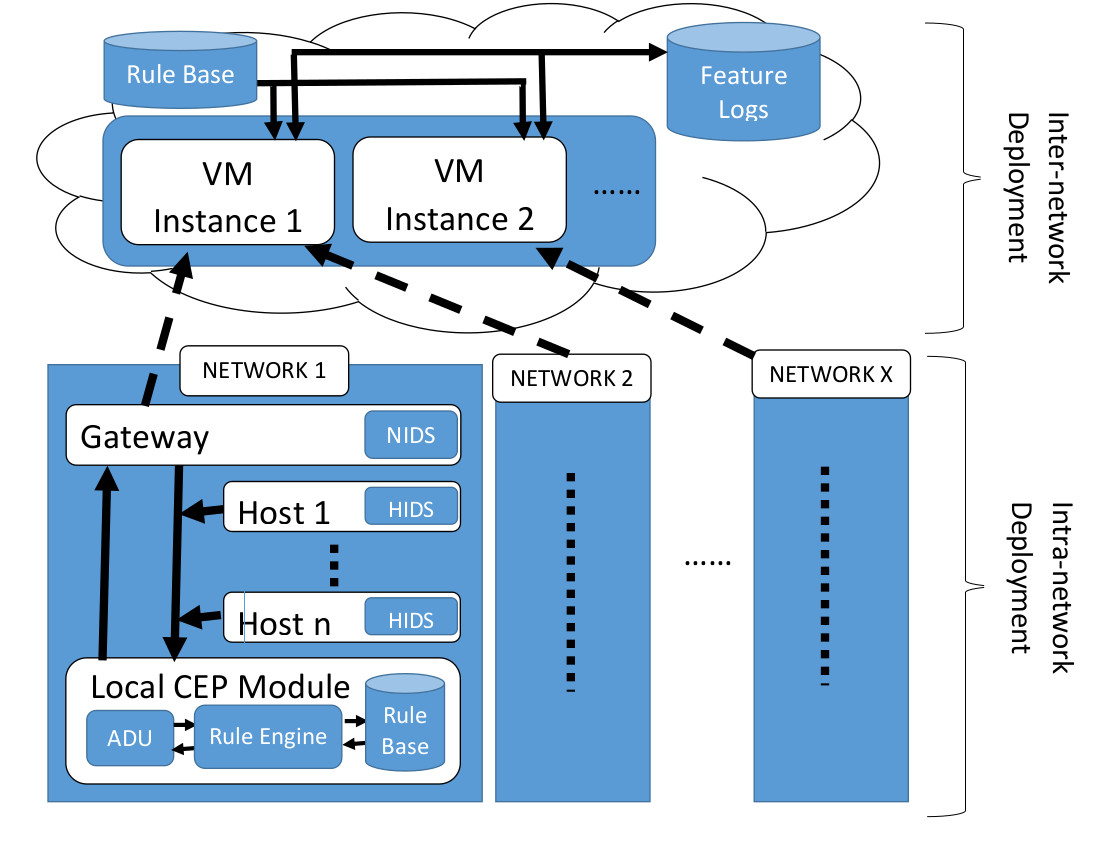
\includegraphics[width=\textwidth]{framework}
\centering
\end{figure*}

\section{Design}\label{subsec:design}
The proposed setup as shown in Fig 1, is divided into two portions based on their deployment:
\subsection{Intra-network Implementation}
  This corresponds to the portion of deployment confined within a single network and consists of:
  \begin{itemize}
    \item \textbf{Network IDS (NIDS)}: The NIDS is placed at the gateway of the network in concern in order to capture all network related traffic at a single point. This deployment extracts features that characterize the network and also detects threats based on a signature based detection module. Additionally, it sends the logged features to the Local CEP Module using Transport Layer Security (TLS) for further analysis and log maintenance.
    \item \textbf{Host IDS (HIDS)}: The HIDS is deployed at each and every host in the network and it closely monitors and logs host-based features to detect threats based on a signature based detection module implemented as a part of it. Besides this, it also sends the captured features to the Local CEP Module using Transport Layer Security (TLS) for further analysis and logging purposes.
    \item \textbf{Local CEP Module}: This module is a separate hardware deployment whose placement is identical to that of a host. It aggregates all the feature updates sent by the HIDs and NIDS of the network in concern and uses anomaly based detection techniques like Multivariate Correlation Analysis (MCA). Additionally, it also uses a rule based detection technique with a wider rule set compared to the NIDS and HIDS to correlate multiple related security incidents that seem independent to each other.
  \end{itemize}
\subsection{Inter-network Implementation}
  This comprises of a deployment that has access to feature information over multiple networks, namely:  
  \begin{itemize}
    \item \textbf{Comprehensive IDS offered as a SaaS (Software as a Service)}
This is deployed as a cloud service. It aggregates the results from various local CEP modules, thus making it an ultimate point of log collection and an apt location for a comprehensive analysis of the collected data to identify sophisticated threats that are not evident from a local networks perspective.
  \end{itemize}

\section{Implementation and Design Decisions}\label{subsec:implementation}
The proposed setup is divided into two portions based on their deployment:
\subsection{Intra-network Implementation}
This setup consists of the following deployments:
\begin{itemize}
  \item \textbf{Network IDS (NIDS)}: 
  In the NIDS module as shown in Figure 1, we implemented a sub-module to extract 16 unique features from the machine on which the NIDS will be deployed on. This was done with the help of a java library called SIGAR - System Information Gatherer and   Reporter \cite{sigar} Additionally, we not only analyze the system features, but also capture and   analyze live network traffic with the help of the jNetPcap library \cite{jnetpcap}. The analysis includes evaluating data from live packets for the purpose of identifying signature based attacks such as (but not limited to) port scan, SYN flood, and land attack. When an attack is detected, an alert flag is set, and the CEP is sent the feature vectors in consideration. The extracted system features will complement the network traffic to identify different anomalies. For E.g. If the RAM usage spikes up and there are 3000 SYN packets being received we can alert the CEP. But if the RAM usage spikes up and there is normal network traffic then it could just be because of some heavy application. The list of extracted features are as follows: 


\begin{enumerate}
  \item System related features
  \begin{itemize}
    \item General Features
      \begin{itemize}
        \item Name of operating system
        \item Version and patch of operating system
        \item Size of the swap space
        \item Firewall status (User group and domain information)
        \item List of all the processes and users responsible for them
        \item List of all the users on the system along with their privileges 
      \end{itemize}
    \item Resource Utilization
      \begin{itemize}
        \item Memory usage in percentage
        \item CPU usage in percentage
        \item Number of bytes being read from the disk
        \item Number of bytes being written to the disk
      \end{itemize}
  \end{itemize}
  \item Network related Features
  \begin{itemize}
    \item List of network adapters with their MAC addresses, IP addresses, downlink and uplink speeds respectively
    \item List of all connections, with packets sent/received, speed, start time/end time, type of connection values for each connection respectively
    \item Deep inspection of packets to find out which application layer protocols are being used
    \item Deep inspection of packets to find out which transport layer protocols are being used
    \item Deep inspection of packets to find study header fields of transport and application layer protocols to gain in-depth knowledge
    \item List of all LAN-external IP addresses
  \end{itemize}
\end{enumerate}
Then, this data will be filtered and sent to the CEP module using Transport Layer Security (TLS). The NIDS module has the additional capability of scanning basic attacks at the end systems so as to avoid transmission overhead. These signature based attacks will be detected at the end user systems itself using SBM, instead of sending the data to CEP and CEP reporting it back to the end users. The Signature Based Model (SBM) has been designed to detect attacks that can easily be observed through packet analysis. Currently, SBM detects three such attacks, Land, SYN-flood, and Port-scan respectively. SBM has been implemented in the following way. First packets captured by the Feature Extraction module are inspected in real time. Packet inspection occurs within a specified time threshold. Upon expiration of the time threshold, data from the analysis is then compared to pre-defined thresholds to detect the possibility of either of the aforementioned attacks. Should an attack be detected, a new Alert object is created, and the alert is subsequently sent to the Update module, and then in turn sent to CEP. To illustrate concretely, SBM serially accesses packets from Feature Extraction for a period of time T. During this time, SBM tallies the number of unacknowledged (no corresponding ACK) SYN flags and the count of unique ports queried. SBM additionally compares Source and Destination IP/Port numbers to detect a potential Land attack. Should Source/Destination IP/Port numbers match, an Alert is immediately sent to the Update module.
Once T has expired, SBM evaluates the live data analysis.  Should the number of unacknowledged SYN flags received be greater than a manually defined threshold value and also 25\% greater than a training (machine learned) value, SBM generates an Alert. Similarly, should the number of unique ports of unacknowledged SYN segments be greater than the manually prescribed threshold value, SBM generates an Alert with the appropriate code. A complete documentation for the Host, Network and Mobile IDS can be found here \cite{javadoc1}.
  \item \textbf{Host IDS (HIDS)}: The HIDS deployment in figure 1.1 is identical to the NIDS deployment and uses jNetPcap for packet capture, SIGAR for local system feature extraction and java serialization to store the Host instances and send them as updates to the local CEP module using Transport Layer Security (TLS).
  \begin{figure*}
\caption{MCA Framework Diagram \cite{MCA}} 
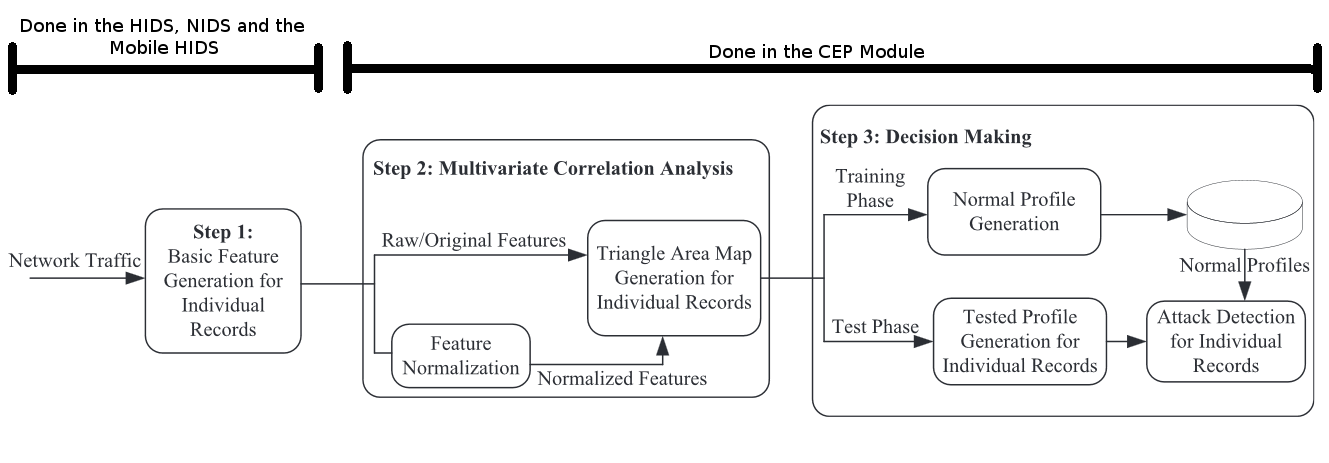
\includegraphics[width=\textwidth]{mcaf}
\centering
\end{figure*}
  \item \textbf{Local CEP Module}: This takes take inputs from host based and network based intrusion detection   systems   and   attempts   to   make correlations   among   these   inputs to classify   abnormal   behavior   resembling a DDoS Attack using the Multivariate Correlation Analysis Technique (MCA) \cite{MCA}. ADU refers to the Anomaly Detection Unit. It houses the MCA Algorithm and other anomaly detection algorithms that are to be implemented can be kept there.
Multivariate Correlation Analysis, in which the triangle area map generation module is applied to extract the correlations between two distinct features within each traffic record.
The MCA implementation as shown in Fig 2 consists of two phases; they are as follows:


\begin{itemize}
  \item \textbf{Training phase} - The normal behavior of the network is characterized here in terms of Mahalanobis Distance and Standard Deviation as shown in Fig 3
  \begin{figure}[H]
\caption{MCA Training Phase \cite{MCA}} 
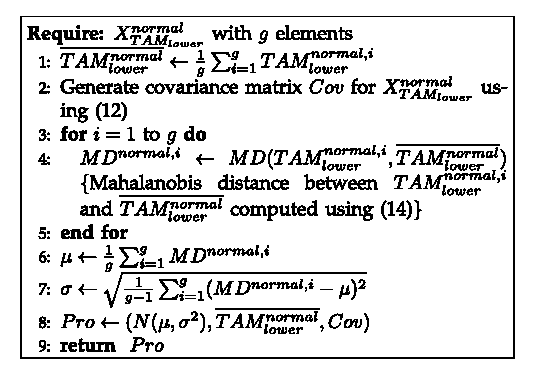
\includegraphics[width=\columnwidth]{mcatrain}
\centering
\end{figure}
  \item \textbf{Testing Phase} - As shown in Fig 4, this phase is used to perform anomaly detection. Classification is done based on the MD and standard deviation computed in the training phase. The feature vectors that lie within the range denoted in step 3 of Fig 4, where alpha is in the range [1,3] for normal distribution, correspond to the normal operation of the network, whereas all outliers in the range are classified as anomalies.
   \begin{figure}[H]
\caption{MCA Testing Phase \cite{MCA}}
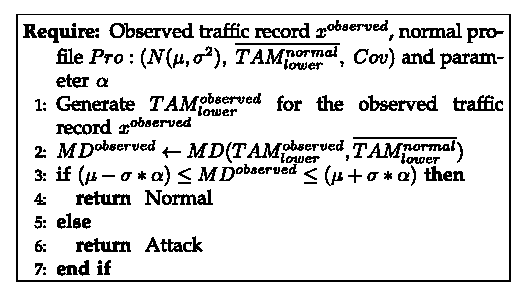
\includegraphics[width=\columnwidth]{mcatst}
\centering
\end{figure}
\end{itemize}



Thus CEP Rule Engine will be able to detect an incoming DDoS and raise alerts in case of any deviation from the normal working state recorded by MCA. Since scalability is a big concern in our project, the MCA class should be able to run multiple instances in a highly efficient manner. We optimized the efficiency of MCA by using better data structures in our design and by minimizing all redundancies. To reduce the time of data encoding and processing, we   decided   to   send   the serialized Host/Network instances \cite{javadoc1} instead of sending feature values. This design simplifies the communication process.
The MCA algorithm is chosen for the following reasons:
The Mahalanobis distance computed as a part of the MCA, yields a better detection accuracy with lower false positives in the dataset used in the reference paper \cite{javadoc2}.
The MCA algorithm detects anomalies that show a linear variation in features as well
The 6\% gureKDD Dataset \cite{gurekdd} is used to evaluate the MCA Algorithm and the details of the attacks present in it are presented in Table 1 and Fig 5. 
In addition to the above mentioned tasks, this local CEP module forwards the received features to the IDS deployed in the cloud for further analysis and log keeping.
\end{itemize}


\begin{figure*}[t]
\caption{Attack Distribution in the 6\% GureKDD Dataset}
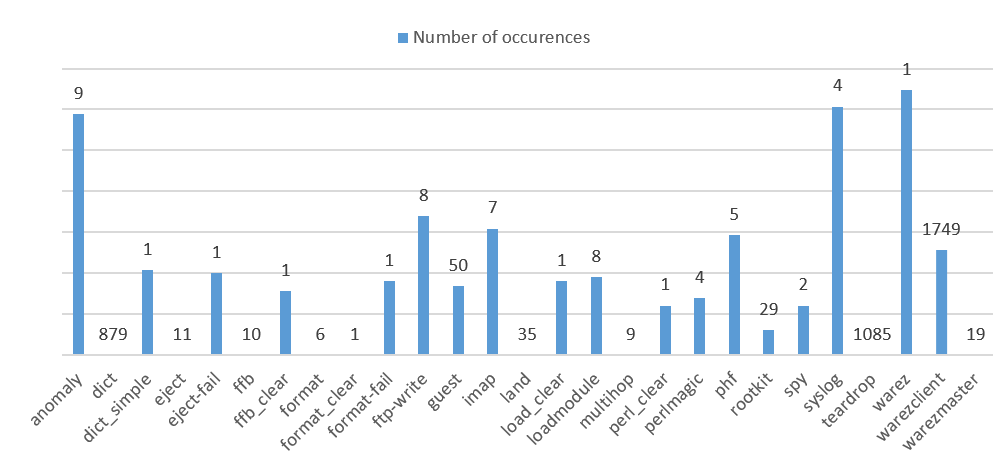
\includegraphics[width=\textwidth]{attack_dist}
\centering
\end{figure*}



\begin{table*}[]
\centering
\caption{List of Attacks present in the 6\% GureKDD Dataset}
\label{my-label}
\begin{tabular}{|cl}
\hline
\textbf{Attack}                     & \multicolumn{1}{|c|}{\textbf{Description}}                                                                                                                                                                                                                                           \\ \hline
\multicolumn{1}{|c|}{anomaly}       & \multicolumn{1}{l|}{\begin{tabular}[c]{@{}l@{}}The identification of items, events or observations which do not\\ 			conform to an expected pattern or other items in a dataset.\end{tabular}}                                                                                     \\ \hline
\multicolumn{1}{|c|}{dict}          & \multicolumn{1}{l|}{\begin{tabular}[c]{@{}l@{}}The Dictionary attack is a Remote to Local User attack in which an\\ 			attacker tries to gain access to some machine by making repeated\\ 			guesses at possible usernames and passwords.\end{tabular}}                            \\ \hline
\multicolumn{1}{|c|}{dict\_simple}  & \multicolumn{1}{l|}{Simple version of dict, just lowercase and check for stopword.}                                                                                                                                                                                                \\ \hline
\multicolumn{1}{|c|}{eject}         & \multicolumn{1}{l|}{\begin{tabular}[c]{@{}l@{}}The Eject attack is a User to Root Attack. It exploits a buffer\\ 			overflow is the 'eject' binary distributed with Solaris 2.5.\end{tabular}}                                                                                     \\ \hline
\multicolumn{1}{|c|}{eject-fail}    & \multicolumn{1}{l|}{A subtype of Eject attack.}                                                                                                                                                                                                                                    \\ \hline
\multicolumn{1}{|c|}{ffb}           & \multicolumn{1}{l|}{\begin{tabular}[c]{@{}l@{}}Ffbconfig attack is a User to Root Attack. It exploits a buffer overflow is\\ 			the 'ffbconfig' program distributed with Solaris 2.5.\end{tabular}}                                                                                \\ \hline
\multicolumn{1}{|c|}{ffb\_clear}    & \multicolumn{1}{l|}{A subtype of Ffbconfig attack.}                                                                                                                                                                                                                                \\ \hline
\multicolumn{1}{|c|}{format}        & \multicolumn{1}{l|}{\begin{tabular}[c]{@{}l@{}}The Fdformat attack is a User to Root Attack. It exploits a buffer\\ 			overflow is the 'fdformat' program distributed with Solaris 2.5.\end{tabular}}                                                                              \\ \hline
\multicolumn{1}{|c|}{format\_clear} & \multicolumn{1}{l|}{A subtype of Fdformat attack.}                                                                                                                                                                                                                                 \\ \hline
\multicolumn{1}{|c|}{format-fail}   & \multicolumn{1}{l|}{A subtype of Fdformat attack.}                                                                                                                                                                                                                                 \\ \hline
\multicolumn{1}{|c|}{ftp-write}     & \multicolumn{1}{l|}{\begin{tabular}[c]{@{}l@{}}The Ftp-write attack is a Remote to Local User attack that takes\\ 			advantage of a common anonymous ftp misconfiguration.\end{tabular}}                                                                                           \\ \hline
\multicolumn{1}{|c|}{guest}         & \multicolumn{1}{l|}{\begin{tabular}[c]{@{}l@{}}The Guest attack is a Remote to User Attack. It is a variant of the\\ 			Dictionary attack.\end{tabular}}                                                                                                                           \\ \hline
\multicolumn{1}{|c|}{imap}          & \multicolumn{1}{l|}{\begin{tabular}[c]{@{}l@{}}The Imap attack is a Remote to Local User attack. It exploits a buffer\\ 			overflow in the Imap server of Redhat Linux 4.2 that allows remote\\ 			attackers to execute arbitrary instructions with root privileges.\end{tabular}} \\ \hline
\multicolumn{1}{|c|}{land}          & \multicolumn{1}{l|}{\begin{tabular}[c]{@{}l@{}}The Land attack is a denial of service attack that is effective\\ 			against some older TCP/IP implementations.\end{tabular}}                                                                                                       \\ \hline
\multicolumn{1}{|c|}{load\_clear}   & \multicolumn{1}{l|}{A subtype of Loadmodule attack.}                                                                                                                                                                                                                               \\ \hline
\multicolumn{1}{|c|}{loadmodule}    & \multicolumn{1}{l|}{\begin{tabular}[c]{@{}l@{}}The Loadmodule attack is a User to Root attack against SunOS 4.1\\ 			systems that use the xnews window system.\end{tabular}}                                                                                                       \\ \hline
\multicolumn{1}{|c|}{multihop}      & \multicolumn{1}{l|}{\begin{tabular}[c]{@{}l@{}}An attack against Multi-hop network. Multi-hop network is a wireless\\ 			networks use two or more wireless hops to convey information from\\ 			a source to a destination.\end{tabular}}                                           \\ \hline
\multicolumn{1}{|c|}{normal}        & \multicolumn{1}{l|}{Normal state.}                                                                                                                                                                                                                                                 \\ \hline
\multicolumn{1}{|c|}{perl\_clear}   & \multicolumn{1}{l|}{A subtype of Perl attack.}                                                                                                                                                                                                                                     \\ \hline
\multicolumn{1}{|c|}{perlmagic}     & \multicolumn{1}{l|}{\begin{tabular}[c]{@{}l@{}}The Perl attack is a User to Root attack that exploits a bug in some\\ 			Perl implementations.\end{tabular}}                                                                                                                       \\ \hline
\multicolumn{1}{|c|}{phf}           & \multicolumn{1}{l|}{\begin{tabular}[c]{@{}l@{}}The phf attack is a Remote to Local Attack that abuses a badly written\\ 			CGI script to execute commands with the privilege level of the\\ 			http server.\end{tabular}}                                                          \\ \hline
\multicolumn{1}{|c|}{rootkit}       & \multicolumn{1}{l|}{\begin{tabular}[c]{@{}l@{}}A rootkit is a clandestine computer program designed to provide\\ 			continued privileged access to a computer while actively hiding\\ 			its presence.\end{tabular}}                                                               \\ \hline
\multicolumn{1}{|c|}{spy}           & \multicolumn{1}{l|}{\begin{tabular}[c]{@{}l@{}}Software that enables a user to obtain covert information about another's\\ 			computer activities by transmitting data covertly from their hard\\ 			drive.\end{tabular}}                                                          \\ \hline
\multicolumn{1}{|c|}{syslog}        & \multicolumn{1}{l|}{\begin{tabular}[c]{@{}l@{}}The Syslogd is a Denial of Service Attacks that exploit is a denial of\\ 			service attack that allows an attacker to remotely kill the\\ 			syslogd service on a Solaris server.\end{tabular}}                                     \\ \hline
\multicolumn{1}{|c|}{teardrop}      & \multicolumn{1}{l|}{\begin{tabular}[c]{@{}l@{}}The teardrop exploit is a denial of service attack that exploits a\\ 			flaw in the implementation of older TCP/IP stacks.\end{tabular}}                                                                                            \\ \hline
\multicolumn{1}{|c|}{warez}         & \multicolumn{1}{l|}{\begin{tabular}[c]{@{}l@{}}During this attack, a warezmaster or warezlicent logs into an anonymous\\ 			FTP site and creates a file of a hidden directory.\end{tabular}}                                                                                       \\ \hline
\multicolumn{1}{|c|}{warezclient}   & \multicolumn{1}{l|}{A subtype of warez attack. Slave portion, compromised and under the control of the master.}  
                                                                                                                                                                                                                                  \\ \hline
\multicolumn{1}{|c|}{warezmaster}   & \multicolumn{1}{l|}{A subtype of warez attack. Master portion, responsible for control.}                                                                                                                                                                                                                                                         \\ \hline
\end{tabular}
\end{table*}


\section{Evaluation}\label{subsec:evaluation}
The evaluation of the proposed implementation have been evaluated as follows:
\subsection{Functional Evaluation}
The functional requirements are evaluated as follows:
\begin{itemize}
  \item \textit{Modularity} - We have successfully achieved the optimal level granularity by splitting the proposed system into subsystems and components to ensure ease of modification. This is achieved by modularizing right from the code level, where we split the work of local deployments among several classes as mentioned in our code documentation \cite{javadoc1,javadoc2}. Aside the code level modularization, using different deployments for Hosts and Networks and the outsourcing of anomaly detection in a network to a local CEP Module and hosting an IDS as a SaaS to aggregate the data from multiple networks represents the deployment level modularization and is done in a way such that the workload is distributed as evenly as possible without compromise in the security and performance of the IDS.
  \item \textit{Cost effectiveness} - The major computing in HIDS/NIDS is done in the feature extraction of 16 unique features and live packet capturing and its local analysis before being sent to the CEP. After multiple runs, we found out that HIDS and NIDS implementation require 5-10\% of CPU (CPU: AMD FX 6300 - Six Core processor @ 3.5 GHz) resources and 250MB to 700MB of RAM. To derive average attack detection time for SBM, the time for SBM to evaluate aggregated data (this value excludes time threshold, described previously in SBM implementation) and subsequently send or not send alerts was calculated over multiple runs. The average was then computed over those time values, yielding an average detection time of 14 milliseconds for SBM.As far as infrastructure deployment it only requires the cloud service and one additional host per network to house the local CEP module. As the providers cloud service hardware configuration can be dynamically varied as per requirement, thus enforcing the concept of pay for exact usage without the requirement to invest in heavy hardware.
  \item \textit{Efficiency} - The feature extraction extracts 16 unique features continuously after certain intervals of time. On average the feature extraction takes only 5 seconds on Windows machines and 4 seconds on Linux machines. Additionally, we monitor the live traffic - incoming and outgoing. This process is continuous with 99\% packet classification accuracy i.e. whether TCP/UDP/ICMP. Since this deployment enforces the heavy computations only on dedicated machines such as the local CEP module and the Cloud Service it does not compromise the performance of user machines on the network. The bottleneck in terms of the deployments efficiency would be the connectivity factors (Latency, Throughput etc).
  \item \textit{Ease of deployment} - For Host and Gateway Machines, with easy to install software it makes it possible to deploy the HIDS and NIDS very efficiently. Also, each HIDS and NIDS copy, once installed, will have a unique identifiers hard-coded which will prevent some adversary machine to masquerade any one of the HIDS or NIDS. Additionally, if a duplicate HIDS/NIDS identifier is found at any point of time, the CEP will generate an alert. Only one dedicated hardware deployment per N/W is needed for the CEP module.
\end{itemize}

\subsection{Security Evaluation}
The security requirements are evaluated as follows:
\begin{itemize}
  \item \textit{SBM Detection} - For each attack in SBM, we used a test bench to evaluate attack detection.  Ostinato software was implemented to simulate Land Attack and SYN-flood.  20 runs were used for each attack.  SBM successfully identified each attack simulation with an accuracy 100\%.  To simulate a Land Attack, packets were formed by Ostinato with the same source/destination IP addresses and source/destination port numbers where SBM correctly identified the malformed packet.  A SYN-flood was created by programming Ostinato to send 100,000 SYN packets at a rate of 100 packets/s.  After an average of 1,294 packets were sent, SBM successfully detected the attack.  Port Scanning was implemented using NMAP stealthy scan.  The stealthy scan simply sends unacknowledged TCP SYN packets to probe the network.  For each scan tested, SBM successfully detected the port scan within one-time threshold of packet inspection.
  \item \textit{Communication Integrity} - Enforcing TLS in all the IDS traffic ensures computationally secure authentication and confidentiality. The rules which constantly monitor for any signs of spoofing also help enforce the communication integrity.
  \item \textit{Cloud reliability and trustworthiness} - The data stored in the cloud is done using SecureDB \cite{securedb} which provides static data confidentiality and can be operated with TLS to ensure authentication over update related connections. Since only the obfuscated executable is deployed in the cloud, it will be infeasible for the adversary to change the change or view the IDS code even if he gains access to the Cloud Deployment. 
  \item \textit{Small Attack Surface / Less Invasiveness} - This deployment is designed keeping in mind to minimize the Network Attack Surface (By enforcing authentication (TLS), confidentiality (TLS) and internal transparency in tunneling in all IDS related communication) and Software Attack Surface (By code obfuscation, not using non-default port numbers for common services used by the IDS deployment, disabling the standard ICMP for IDS related deployments and using a custom version of ICMP).
  \item \textit{Need based rules} - The proposed model pulls rules from the cloud based deployment based on the alerts detected. This increases the chances of related attacks being detected at a much earlier stage and in a much more efficient manner. For example, if a particular set of hosts show excessive power usage, then the appropriate power based DoS attack rules are pulled from the cloud for verification at the CEP end.
  \item \textit{Detection Accuracy of MCA} - The MCA Algorithm was trained for 10000 records and tested over 178810 records in the 6\% gureKDD dataset \cite{ddos}. The results obtained were as shown in Table 2.
  \begin{center}
  \begin{table}[H]
  \centering
  \caption{List of Attacks present in the 6\% GureKDD Dataset}
  \begin{tabular}{ | c | p{1.5cm} | p{1.5cm} | p{1.5cm} | }
    \hline
     & Detection Accuracy & False Positive & False Negatives \\ \hline
    Count & 174873 & 0 & 3937 \\ \hline 
    Percentage & 97.7982 & 0 & 2.2018 \\  \hline
  \end{tabular}
  \end{table}
\end{center}
\end{itemize}
Considering the above stated facts in terms of making use of computationally secure authentication and confidentiality in communication and storage with minimum attack surface, it considerably minimizes the chances of this model being exploited.

\section{Related Work}\label{subsec:relatedwork}
Extensive research has been conducted to improve the scalability of IDS. Various approaches to this problem have been proposed. E.g. Privacy-Preserving Signature-based IDSaaS \cite{IDSaaS}, Parallel design for Network Intrusion Detection Systems \cite{multicore}, and CEP-based IDS for Internet of Things \cite{CEP2}.
In the Privacy-Preserving Signature-based IDSaaS \cite{IDSaaS}, cloud computing can provide IDS capabilities such as monitoring and logging suspicious network behaviors between virtual machines and users. The major advantages of cloud-based IDS are scalability and availability. Users can scale the service based on their demand, and can rely on cloud provider for availability. The main difference of this system and other IDSaaS is that it is a privacy-preserving IDS, which means a cloud provider will not be able to learn any sensitive data during the packet inspection. Thus, the system is still secure in scenarios where the cloud provider goes rouge. This paper focuses uses IDSaaS mainly for offloading the expensive operations, while we propose to use IDSaaS for scalability and as well as offloading.
In Parallel design for Network Intrusion Detection Systems \cite{multicore}, TILERAGX36 Processor (a 36-core processor) is used to speed up the detection engine. In this design, they exploit the computational power of many-core processors by using a parallel architecture that combines both data and pipeline parallelism. Each packet is processed in separate cores and the packet processing is divided into several sequential stages. Their experiments showed almost linear speedup and can handle up to 7.2 Gbps traffic with 100-bytes packets. This paper only discusses improving performance of IDS which is directly dependent on the hardware. On the other hand, we implement a system which can handle similar data even without 36-core processors, due to the IDSaaS idea.  
In CEP-based IDS for Internet of Things \cite{CEP2}, authors demonstrate that CEP mechanism is more suitable for applications and services which need to process large among of data. One useful strategy we adapted from this design is that by using relational database for rules, we can improve the efficiency of rule searching. For our project, relational database for rules can also avoid data duplication and inconsistent record.
Finally, we studied a paper \cite{hybrid}, where the authors propose a novel hybrid detection system referred to as H-IDS, which is comprised of anomaly-based and signature-based detection techniques for more accurate DDoS attack detection. Their proposed detection system can be adopted to various networks with varying traffic patterns due to the flexibility provided through the used decision combiner and the associated sensitivity parameter. They have tested the proposed systems performance against systems based on non-hybrid detection by using two distinct datasets (DARPA and a commercial bank penetration test). The results are satisfactory, which shows that the proposed hybrid system can be an efficient solution in the DDoS detection process. They also found out that some sophisticated DDoS attacks may evade the signature-based detector rules, which are commonly known, and the system performance may decrease as the detection success solely depends on the anomaly detector. Also the training need of anomaly detector stands as a limitation on the overall system performance. The training data may not reflect the real network model in a practical system or even may be unavailable, which may result in decreased performance. We use a better algorithm called MCA which overcomes this problem.

\section{Future Work}\label{sec:futurework}
We have implemented a full-fledged working system for a local network. We have proposed the extension of this system which would be scalable as well as secure. Future work would include the following:
\begin{itemize}
  \item Adding full-fledged TLS Support for all IDS related communication.
  \item IDSaaS Implementation
\end{itemize}

\section{Concluding Remarks}\label{sec:concludingremarks}
We have implemented Host IDS (HIDS) and Local CEP Module of this effective and scalable hybrid IDS design and have also proposed a generic hybrid IDS design to bring forth a standardization in the IDS Framework portion of the computer security domain and to evaluate it in terms of performance and security. Implementation of Network IDS (NIDS) is partially complete and we project that it will have been done till the next report. All the modules have been tested independently but testing and evaluation as a whole system is yet to be done. Comprehensive IDS offered as a SaaS (Software as a Service) is proposed for exploring the IDS design space and is part of future work.



\begin{thebibliography}{9}
\bibitem{CEP1} 
R. Mohan, V. Vaidehi, A. Krishna, M. M, S. S. Chakkaravarthy and R. Pathak. 
\textit{Complex Event Processing Based Hybrid Intrusion Detection System}. 
3rd International Conference on Signal Processing, Communication and Networking (ICSCN), Chennai, 2015.

\bibitem{MCA} 
Z. Tan, A. Jamdagni, X. He, P. Nanda and P. R. Liu.
\textit{A System for Denial-of-Service Attack Detection Based on Multivariate Correlation Analysis}. 
IEEE Transactions on Parallel and Distributed Systems, 2014.
  
\bibitem{IDSaaS} 
Y. Meng.
\textit{Towards Designing Privacy-Preserving Signature-based IDS as a Service: A Study and Practice}. 
5th International Conference on Intelligent Networking and Collaborative Systems (INCoS), 2013.

\bibitem{multicore} 
H. Jiang.
\textit{Scalable High-Performance Parallel Design for Network Intrusion Detection Systems on Many-Core Processors}. 
ACM/IEEE Symposium on Architectures for Networking and Communications Systems (ANCS), 2013.

\bibitem{CEP2} 
C. Jun.
\textit{Design of Complex Event-Processing IDS in Internet of Things}. 
Sixth International Conference on Measuring Technology and Mechatronics Automation, 2014.

\bibitem{hybrid} 
O. Cepheli, S. Buyukcorak and K. G. Kurt.
\textit{Hybrid Intrusion Detection System for DDoS Attacks}. 
Journal of Electrical and Computer Engineering, 2016.

\bibitem{sigar} 
System Information Gatherer and Reporter.
\\\texttt{http://support.hyperic.com/display/SIGAR/Home}

\bibitem{javadoc1} 
Host and N/W IDS Documentation.
\\\texttt{http://goo.gl/2ESffv}

\bibitem{serialization} 
Java Serialization.
\\\texttt{http://tutorialspoint.com/java/java\_serialization.htm}

\bibitem{securedb}
SecureDB
\\\texttt{https://securedb.co}

\bibitem{drools}
jDrools Complex Event Processing Engine
\\\texttt{http://drools.org}

\bibitem{jama}
Java Matrix Package
\\\texttt{http://math.nist.gov/javanumerics/jama}

\bibitem{ddos}
DDoS Datasets
\\\texttt{http://si.edu/ant/traces/dataset\_list.html}

\bibitem{jnetpcap}
jNet Pcap
\\\texttt{http://jnetpcap.com}

\bibitem{javadoc2}
CEP Module Documentation
\\\texttt{http://goo.gl/wLxChh}

\bibitem{template}
Gentella Admin Template
\\\texttt{http://colorlib.com/polygon/gentella}

\bibitem{jersey}
Jersey Web Services
\\\texttt{https://jersey.java.net/}

\bibitem{maven}
Maven Build Tool
\\\texttt{https://maven.apache.org/}

\bibitem{gurekdd}
GureKDD Dataset
\\\texttt{http://www.aldapa.eus/res/gureKddcup/}



\end{thebibliography}



\end{document}
